\documentclass{memoir}
\usepackage{fdvs-style}

\begin{document}

\setcounter{section}{20}
\section{Determinants}

\begin{dfn} \mbox{}
\begin{enumerate*}
\item Let $V_i$ and $W$ be vector spaces and let $n$ be a positive integer. A mapping \[f : \underbracket{V_1 \times \cdots \times V_n}_{t\ \text{times}} \rightarrow W\] is called \emph{multilinear} if $f$ is linear in each slot. That is, for each $j$, if $v_i \in V_i$ are fixed ($i \neq j$) then the map \[ x \mapsto f(v_1,\ldots,v_{j-1}, x, v_{j+1},\ldots,v_n) \] is a linear transformation. For $n=2,3$, we say \emph{bilinear} and \emph{trilinear}, respectively. We say $f$ is \emph{alternating} if $f(v_1,\ldots,v_n) = 0$ anytime $v_i=v_{i+1}$ for some $i$ (i.e. two consecutive inputs are equal).
\item Let $n$ be a natural number and $V = \Mat{n}{1}{F}$. An $n$-linear alternating function \[f : \underbracket{V \times \cdots \times V}_{n\ \text{times}} \rightarrow F\] is called a \emph{determinant} if $f(d_1,d_2,\ldots,d_n) = 1$, where $d_i$ denote the standard basis vectors.
\end{enumerate*}
\end{dfn}

\begin{prp}
For each $n$ and $F$, there is a unique determinant function. In fact, it can be computed explicitly by the following formula. \[ \left( \begin{bmatrix} \alpha_{1,1} \\ \alpha_{2,1} \\ \vdots \\ \alpha_{n,1} \end{bmatrix}, \begin{bmatrix} \alpha_{1,2} \\ \alpha_{2,2} \\ \vdots \\ \alpha_{n,2} \end{bmatrix}, \cdots, \begin{bmatrix} \alpha_{1,n} \\ \alpha_{2,n} \\ \vdots \\ \alpha_{n,n} \end{bmatrix} \right) \mapsto \sum_{\sigma \in S_n} \Sign{\sigma} \prod_{i=1}^n \alpha_{\sigma(i),i} \] where $S_n$ denotes the symmetric group on $\intrange{1}{n}$ and $\Sign{\sigma}$ is the sign of the permutation $\sigma$.
\end{prp}

Of course given a square matrix $M$, the determinant of $M$ is the value of this function as applied to the columns of $A$. This leads to a natural computational question: Given a matrix $M$, what is $\Det{M}$? And from a computational complexity point of view, how difficult is it to compute $\Det{M}$? The formula above certainly is one way to do it. However, it requires computing a sum over all the permutations of $\intrange{1}{n}$, of which there are $n!$. There are other ways: one, a recursive strategy called \emph{cofactor expansion}, still requires about $n!$ steps in the worst case but is useful by hand on matrices with lots of zeros; and another, which factors $A$ as a product of elementary matrices by row reduction and uses the following fact about determinants, and takes about $n^3$ steps.

\begin{prp} \mbox{}
\begin{enumerate*}
\item $\Det{A^\mathsf{T}} = \Det{A}$
\item $\Det{AB} = \Det{A} \Det{B}$.
\item If $P$ is invertible, then $\Det{P^\inv} = \Det{P}^\inv$.
\item A matrix $A$ is nonsingular (i.e. is invertible) if and only if $\Det{A} \neq 0$.
\end{enumerate*}
\end{prp}

\begin{dfn} \mbox{}
\begin{enumerate*}
\item Let $\varphi : V \rightarrow V$ be a linear transformation and let $\lambda \in F$. We say that $\lambda$ is an \emph{eigenvalue} if $E_\lambda = \Ker{\lambda 1 - \varphi}$ is nontrivial. In this case we call $E_\lambda$ the \emph{eigenspace} of $\varphi$ with eigenvalue $\lambda$, and nonzero elements of $E_\lambda$ are called \emph{eigenvectors}.
\item Given an $n \times n$ matrix $M$, the \emph{characteristic polynomial} of $M$ is $\CharPoly{M}(x) = \Det{xI - M}$. This is indeed a polynomial, and in fact is monic of degree $n$. The roots of $\CharPoly{M}$ are precisely the eigenvalues of $M$. (Note that $F$ need not contain all of the eigenvalues of $M$.)
\end{enumerate*}
\end{dfn}

\begin{prp}
Given an $n \times n$ matrix $M$, we have the following.
\begin{enumerate*}
\item $\MinPoly!{M} \mid \CharPoly{M}$ (This is called the Cayley-Hamilton Theorem)
\item $\CharPoly{M}$ is the product of the invariant factors of $M$.
\item $\CharPoly{M}$ is the product of the elementary divisors of $M$.
\end{enumerate*}
\end{prp}

\section{Tensor Products}

\begin{dfn}
Let $V$ and $W$ be vector spaces over a field $F$, and let $\Free{V \times W}$ denote the free $F$-vector space on the set $V \times W$. We define the subspace $U \subseteq \Free{V \times W}$ to be
\begin{eqnarray*}
U & = & \Span{(v,w_1+w_2) - (v,w_1) - (v,w_2) \mid v \in V, w_1,w_2 \in W} \\
  &   & + \Span{(v_1+v_2,w) - (v_1,w) - (v_2,w) \mid v_1,v_2 \in V, w \in W} \\
  &   & + \Span{(\alpha v, w) - \alpha (v, w) \mid v \in V, w \in W, \alpha \in F} \\
  &   & + \Span{(v, \alpha w) - \alpha (v, w) \mid v \in V, w \in W, \alpha \in F}.
\end{eqnarray*}
The \emph{tensor product} of $V$ and $W$ is the vector space \[ V \otimes_F W = \Free{V \times W}/U. \] The coset $(v,w) + U$ will be denoted $v \otimes w$.
\end{dfn}

One way to think of the tensor product is as a vector space of ``products'' of elements of $V$ and $W$. Suppose for a moment that we are convinced the tensor product of vector spaces is interesting. Having been described as a quotient of a free vector space, defining linear transformations \emph{from} a tensor product directly, or even using the First Isomorphism Theorem, is awkward.

\begin{prp}[Universal Property of Tensor Products]
Let $V$, $W$, and $U$ be vector spaces. If $f : V \times W \rightarrow U$ is a bilinear map, then there is a unique linear transformation $\varphi : V \otimes_F W \rightarrow U$ such that $\varphi(v \otimes w) = f(v,w)$. That is, a unique $\varphi$ such that the following diagram commutes.

\begin{center}
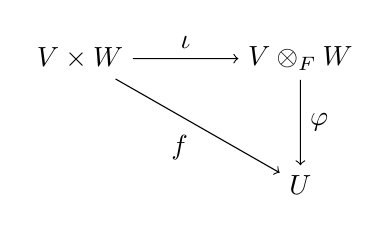
\begin{tikzpicture}[scale=0.8]
  \node (VxW) at (-1.5,2) {$V \times W$};
  \node (VoW) at (2,2) {$V \otimes_F W$};
  \node (U) at (2,0) {$U$};
  \draw[->] (VxW) edge node [above] {$\iota$} (VoW);
  \draw[->] (VxW) edge node [below left] {$f$} (U);
  \draw[->] (VoW) edge node [right] {$\varphi$} (U);
\end{tikzpicture}
\end{center}
\end{prp}

\begin{prp} \mbox{}
\begin{enumerate*}
\item $V \otimes 0 = 0$
\item $V \otimes W \cong W \otimes V$
\item $V \otimes (W \otimes U) \cong (V \otimes W) \otimes U$
\item $V \otimes (W \oplus U) \cong (V \otimes W) \oplus (V \otimes U)$
\item $\Hom{V \otimes W}{U} \cong \Hom{V}{\Hom{W}{U}}$ (vector space theoretic currying)
\item We call the iterated tensor product $\TensorPow{n}{V} = \underbracket{V \otimes \cdots \otimes V}_{n\ \text{times}}$ the $n$th \emph{tensor power} of $V$. Then the map $t_{m,n} : \TensorPow{m}{V} \times \TensorPow{n}{V} \rightarrow \TensorPow{m+n}{V}$ given by $(v,w) \mapsto v \otimes w$ is bilinear.
\end{enumerate*}
\end{prp}

\begin{prp}
If $V$ and $W$ have bases $\mathcal{B}$ and $\mathcal{E}$, respectively, then $\mathcal{B} \otimes \mathcal{E} = \{b \otimes e \mid b \in \mathcal{B}, e \in \mathcal{E}\}$ is a basis for $V \otimes W$. In particular, if $V$ and $W$ are finite dimensional, then so is $V \otimes W$, and in fact $\Dim{V \otimes W} = \Dim{V}\Dim{W}$.
\end{prp}

\end{document}